\chapter{Esperimenti}
\label{cap:esperimenti}
Dopo aver eseguito una prima fase di analisi nel Capitolo~\ref{cap:analisi}, adesso andiamo a descrivere gli esperimenti e i risultati a cui questi portano. Di rilievo sarà la descrizione del representation bias.

\myskip

Quando si esegue un esperimento è necessario, oltre ad avere a disposizione il file di log \textit{trace.log}, definire solo il representation bias. È stato infatti pensato uno script, che dovrà essere modificato in base all'esperimento e trovarsi nella cartella, che legge il file di log e definisce i file tipici di Popper (e quindi di Numsynth) \textit{bk.pl} e \textit{exs.pl} necessarie per il sistema.

Una volta che abbiamo definito una cartella per l'esperimento contenente un file \textit{bias.pl} e uno di log \textit{trace.log}, possiamo lanciare l'esperimento dalla root directory con \texttt{./numsynth.sh <folder-name>}.

%%%%%%%%%%%%%%%%%%%%%%%%%%%%%%%%%%%%%%%%%
\section{Primo approccio}
\label{sec:primo-approccio}
Il primo approccio tentato è stato il più semplice possibile: abbiamo inserito all'interno del representation bias solo quei predicati che rappresentano ciò che i log del simulatore di taskset mostra. Questi nello specifico sono: rilascio e completamento di un task; inizio e fine dell'esecuzione di un chunk. Nella cartella \textit{my-experiments} questo esperimento è \href{https://github.com/edoardosarri24/numsynth/tree/main/my-experiments/1-start/}{start}.

In questo modo stiamo chiedendo al sistema di spiegarci il fallimento o il successo della traccia su cui facciamo inferenza solamente tramite questi predicati. Sarà poi Numsynth a cercare di trovare delle relazioni, anche numeriche, tra chunk e task per coprire il maggior numero di esempi positivi e non coprire nessuno di quelli positivi.

\subsection{Modello}
\label{subsec:mod-primo-approccio}
Ogni traccia in questo esperimento ha una durata di massimo 100ms e sono state generate 100 tracce, di cui 72 hanno terminato con successo e 28 fallendo.

\myskip

Il modello usato per questo esperimento, essendo il primo, è stato semplice e forse banale. È stato usato Rate Monotonic (RM) come algoritmo di scheduling e il taskset ha queste caratteristiche:
\begin{itemize}
    \item Task1: periodo 3ms; deadline relativa 3ms; chunk1 con execution time campionato da un ConstantSampler con parametro 1ms; chunk2 con execution time campionato da un UniformSampler con parametri 0.5ms e 1.1.
    \item Task2: periodo 5ms; deadline relativa 5ms; chunk1 con execution time campionato da un ConstantSampler con parametro 1ms.
\end{itemize}

\subsection{Risultati}
I risultati, che possiamo osservare nel file \href{https://github.com/edoardosarri24/numsynth/tree/main/my-experiments/1-start/result.txt}{result.txt}, mostrano la semplicità del modello scelto per questo esperimento.
\begin{itemize}
    \item Il tempo di addestramento è di circa 14s.
    \item La precision e la recall sono entrambe massime e pari a 1. Questo significa che sono stati coperti tutti gli esempi negativi e nessuno di quelli positivi.
    \item La soluzione è composta da quattro letterali: \texttt{failure(A):-execute(A,D,B,F), \allowbreak finish(A,C,B,F),mult(C,99,D)}.
\end{itemize}

\myskip

La soluzione che il sistema ha trovato ci porta a dei ragionamenti che ne evidenziano le problematiche.

In primo luogo la generalizzazione è molto bassa. Il sistema ha trovato una regola che è il massimo dei True Positive (TP) e il massimo dei True Negative (TN); probabilmente su log più complessi questa regola non riuscirà a prevedere il fallimento della traccia in modo corretto.

Dalla regola appresa possiamo vedere come il sistema classifica una traccia come corretta in base alla sua lunghezza. Nello specifico infatti la traccia ha successo se esiste un chunk \textit{BF} che esegue al tempo \textit{D} e termina al tempo \textit{C}, dove $D=C\cdot100$. Siccome 100 è il massimo valore di una simulazione (i.e., il tempo massimo in una traccia), se una traccia fallisce allora sicuramente non arriva al tempo 100.

Per confermare quanto osservato è stato fatto l'esperimento \href{https://github.com/edoardosarri24/numsynth/tree/main/my-experiments/2-start250/}{start250}, identico al precedente tranne che per la lunghezza delle tracce che è stata portata fino a 250ms. Tra le varie informazioni del file \href{https://github.com/edoardosarri24/numsynth/tree/main/my-experiments/2-start250/result.txt}{result.txt} possiamo osservare quanto previsto: la regola imparata è \texttt{failure(A):- finish(A,B,E,D),execute(A,C,E,D),mult(B,246,C)}, che ci conferma quanto ipotizzato.

%%%%%%%%%%%%%%%%%%%%%%%%%%%%%%%%%%%%%%%%%
\section{Inversione dei positivi e negativi}
\label{sec:posNeg-inversion}
Per cercare di impedire al sistema di utilizzare la lunghezza delle tracce come criterio per valutare la corretterzza di una traccia, sono stati invertiti gli esempi positivi e negativi, lasciando tutto il resto come descritto nella Sezione~\ref{subsec:mod-primo-approccio}, ed è stato così prodotto l'esperimento \href{https://github.com/edoardosarri24/numsynth/tree/main/my-experiments/3-posNeg-inversion}{posNeg-inversion}.

In questo modo il sistema dovrà cercare di spiegare come mai una traccia fallisce e non perché ha successo; non dovrebbe quindi usare la lunghezza della traccia come parametro fondamentale, visto che il fallimento potrebbe avvenire all'inizio della traccia, ma anche un attimo prima del tempo massimo della simulazione.

\subsection{Risultati}
Il risultato di questo esperimento, come si può vedere nel file \href{https://github.com/edoardosarri24/numsynth/tree/main/my-experiments/3-posNeg-inversion/result.txt}{result.txt}, mostra come i predicati descritti fino a questo momento nel representation bias (i.e., il file \textit{bias.pl}) non sono sufficienti. Infatti il sistema non riesce a trovare una soluzione che abbia una precisione e una recall accettabili.

Inoltre, come si spiega nel paper~\cite{numsynth}, per ogni task di ricerca è predisposto un timer di 600s che permette al sistema di entrare in un loop. Questo timer in questo caso viene superato e la ricerca si arresta durante la ricerca di una soluzione con cinque letterali.

%%%%%%%%%%%%%%%%%%%%%%%%%%%%%%%%%%%%%%%%%
\section{Without multiplications}
\label{sec:wo-mult}
Per cercare di evitare che il sistema utilizzi le moltiplicazioni per spiegare il fallimento o il successo di una traccia, gli è stata levata la possibilità di utilizzare le moltiplicazioni nell'esperimento \href{https://github.com/edoardosarri24/numsynth/tree/main/my-experiments/4-wo-mult/}{wo-mult}.

Il modello utilizzato è sempre quello del primo esperimento descritto nella Sezione~\ref{subsec:mod-primo-approccio}. L'unica modifica che è stata portata è quella di eliminare le moltiplicazioni dal representation bias.

\subsection{Risultati}
La prima cosa interessante è notare come il sistema non abbia trovato una soluzione di dimensione quattro, cosa che invece succede nell'omonimo esperimento con la moltiplicazione come predicato utilizzabile.

La seconda cosa che è chiara è che il sistema non riesce a gestire l'elevata ricorsione e quindi la ricerca della soluzione fallisce.

\myskip

Il risultato finale, che possiamo osservare nel file \href{https://github.com/edoardosarri24/numsynth/tree/main/my-experiments/4-wo-mult/result.txt}{result.txt}, ci fornisce due spunti molto importanti:
\begin{itemize}
    \item Senza moltiplicazioni non si si riesce a spiegare il fallimento con una regola che abbia sia un'alta precision che un'alta recall.
    \item Senza predicati aggiuntivi, l'unico modo di spiegare il successo di una traccia in modo efficace (i.e., con un'alta precision e recall) è tramite la sua lunghezza.
\end{itemize}

%%%%%%%%%%%%%%%%%%%%%%%%%%%%%%%%%%%%%%%%%
\section{Magic Popper}
\label{sec:magic-popper}
Come abbiamo detto nella Sezione~\ref{sec:numsynth}, Numsynth estende Popper con i predicati numerici. Oltre a questo permette anche di utilizzare le caratteristiche di MagicPopper~\cite{hocquette2023learning}, cioè permette di far si che in una soluzione non compaiano solamente valori presenti nella background knowledge, ma anche valori inventati.

Da questa idea nasce l'esperimento \href{https://github.com/edoardosarri24/numsynth/tree/main/my-experiments/5-magic/}{magic}. La configurazione è esattamente la stessa di quello senza la moltiplicazione presentato nella Sezione~\ref{sec:wo-mult}; nel representation bias è stato aggiunto \texttt{magic\_value\_type(int)} che permette a Numsynth di inventare valori per il tipo intero, cioè per il tempo.

\subsection{Risultati}
I risultati ottenuti sono esattamente quelli attesi. La regola trovata è \texttt{failure(A):- release(A,95000,D),release(A,0,D)} e ci mostra quanto il sistema si basi sulla lunghezza delle regole per classificarle.

Essa infatti ci dice che, perchè una traccia abbia successo, deve esistere un task \textit{D} che viene rilasciato sia al tempo 0 che al tempo 95000, che praticamente è quasi il tempo massimo che una traccia può durare (100ms).

Ovviamente questo non è quanto vogliamo e ci dice ancora di più che i predicati attuali non sono sufficienti.

%%%%%%%%%%%%%%%%%%%%%%%%%%%%%%%%%%%%%%%%%
\section{Descrittività predicati}
\label{sec:event_task_chunk}
Adesso analiziamo quegli esperimenti che realizzano l'idea descritta nella Sezione~\ref{sec:gestione-task}: vogliamo spiegare il fallimento di una traccia correlando l'evento al task che ha provocato la deadline miss.

Il modello utilizzato è ancora una volta quello base descritto nel primo esperimento nella Sezione~\ref{sec:primo-approccio}.

\myskip

Per lavorare sui predicati, è stato modificato lo script che genera i file \textit{bk.pl} e \textit{exs.pl}. Il risultato adesso è che per ogni predicato \texttt{body\_pred(event,3)} o \texttt{body\_pred(event,4)} sono stati generati tanti predicati \texttt{body\_pred\_taskID(event,2)} o \\ \texttt{body\_pred\_taskID\_chunkID(event,2)} quanti sono i task e chunk, dove le due variabili del predicato sono l'ID della traccia e il tempo in cui l'evento è stato generato.

\subsection{Successo}
Nell'esperimento \href{https://github.com/edoardosarri24/prediction-in-data-driven-system/6-event-task-chunk/}{event-task-chunk} si è cercato di spiegare il motivo del successo di una traccia usando i predicati che descrivono sia l'evento che il chunk (e il relativo task) che lo ha generato.

I risultati sono stati deludenti per un motivo molto semplice: aggiungere il task che ha generato l'evento non impedisce al sistema di utilizzare la lunghezza della traccia per spiegare il suo successo. In realtà il risultato ottenuto è forse peggiore: la regola \texttt{failure(A):- mult(B,99,C),finish\_1\_1(A,B),release\_1(A,C)}, che ha precision e recall massime, attribuisce il successo di una futura traccia su cui faremo inferenza solamente al Task1, considerando il suo rilascio e la fine dell'esecuzione di uno dei suoi chunk.

\subsection{Fallimento}
Nell'esperimento \href{https://github.com/edoardosarri24/prediction-in-data-driven-system/7-event-task-inversion/}{event-task-inversion} si è invece cercato di spiegare il fallimento di una traccia usando i predicati che descrivono sia l'evento che il task che lo ha generato.

Il risultato non è soddisfacente: se osserviamo il file \href{https://github.com/edoardosarri24/prediction-in-data-driven-system/7-event-task-chunk-inversion/result.txt}{result.txt} vediamo chiaramente che la recall della soluzione è molto bassa, e questo vuol dire che il numero di esempi non coperti dalla regola è molto basso. Questo ci testimonia il fatto che con i predicati attuali non riusciamo a spiegare il fallimento di una traccia.

%%%%%%%%%%%%%%%%%%%%%%%%%%%%%%%%%%%%%%%%%
\section{Tempi di esecuzione dei chunk}
\label{sec:execution_time}
Fino a questo momento abbiamo capito che il sistema cerca di spiegare i successi tramite la lunghezza delle tracce e che con i predicati attuali non riusciamo a ottenere una spiegazione che abbia una buona copertura degli esempi.

Da ora in poi eseguiremo gli esperimenti senza moltiplicazioni: non ci sono motivi infatti per cui il fallimento (ma anche il successo) di una traccia debba dipendere dal prodotto di tempi.

Inoltre non considereremo più il successo di una traccia, ma cercheremo solo di spiegarne il fallimento. Per fare questo dobbiamo aggiungere dei predicati che il sistema possa usare.

\subsection{Modello}
L'obiettivo in questo momento è cercare di capire se il sistema impara una regola corretta: ci serve un modello di taskset di cui sappiamo a priori il motivo del fallimento. Il taskset considerato ha le seguenti caratteristiche:
\begin{itemize}
    \item Task1: periodo e deadline di 2ms. Il primo chunk esegue sempre per 0.5ms, il secondo campiona 0.5ms con probabilità del 95\%, 1ms con probabilità complementare.
    \item Task2: periodo e deadline di 4ms. L'unico chunk ha tempo di esecuzione di 2ms.
\end{itemize}
La normale esecuzione del taskset, cioè quella che non porta a fallimento è mostrata in Figura~\ref{fig:tasksetmodel}. In questo modo è chiaro che il taskset fallisce, a causa del Task2, quando il secondo chunk del primo task campiona un tempo di esecuzione di 1ms invece che di 0.5ms.
\begin{figure}[htbp]
    \centering
    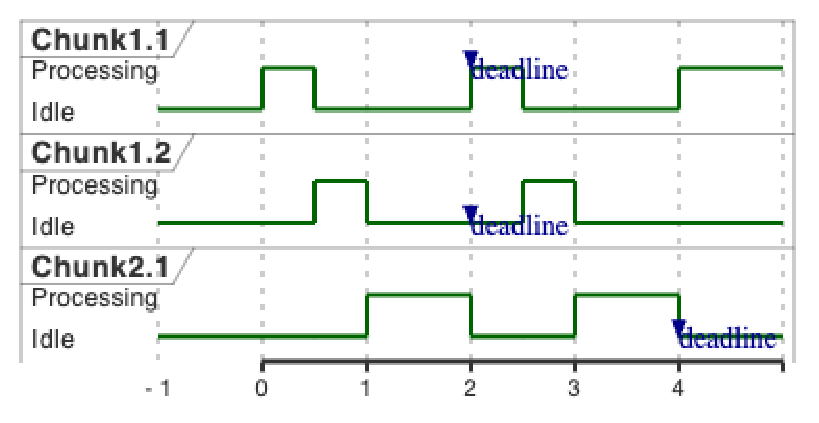
\includegraphics[width=.75\textwidth]{images/3-esperimenti/tasksetmodel.pdf}
    \caption{Normal execution of taskset.}
    \label{fig:tasksetmodel}
\end{figure}

\subsection{Predicati}
Per questo esperimento, oltre ad eliminare le moltiplicazioni come abbiamo detto sopra, sono stati aggiunti i predicati che modellano il tempo di esecuzione di ogni chunk. Questo dovrebbe permettere al sistema di capire come il tempo di esecuzione è responsabile del fallimento di una traccia.

Per implementare questi predicati non è stato toccato il file di log ma è stato modificato lo script che genera \textit{bias.pl}, \textit{bk.pl} e \textit{exs.pl}.

\subsection{Risultati}
Per capire se quanto supposto funzionasse, in un primo momento sono state considerate solo 10 tracce, di cui 9 fallivano e 1 aveva successo. L'esperimento \href{https://github.com/edoardosarri24/prediction-in-data-driven-system/8-executionTime-10traces/}{executionTime-10traces} ha dato esattamente la soluzione che ci aspettavamo: \texttt{failure(A):- \\ executionTime\_1\_2(A,C),geq(C,501)}: questo ci dice esattamente che se il tempo di esecuzione del Chunk1.2 (i.e., il secondo del primo task) campiona un valore superiore di 0.5ms allora la traccia fallisce.

\subsection{Complessità}
La nostra idea funziona, ma dobbiamo testarla su un dataset di tracce maggiore.

Nell'esperimento \href{https://github.com/edoardosarri24/prediction-in-data-driven-system/9-executionTime-100traces/}{executionTime-100traces} sono state testate 100 tracce, di cui 18 falliscono e 82 hanno successo. In questo caso il sistema trova la soluzione \texttt{failure(A):- executionTime\_1\_2(A,C),geq(C,501).}, che è ancora esattamente quella attesa.

Se però usiamo lo stesso numero di tracce, ma il numero di fallimenti, e quindi di esempi da spiegare, aumenta, allora il timeout scatta e non troviamo nessuna soluzione. Queste è infatti quello successo nell'esperimento \href{https://github.com/edoardosarri24/prediction-in-data-driven-system/10-executionTime-100traces-morefailures/}{executionTime-100traces-morefailures}, dove sono le tracce che falliscono sono 27.

L'ultimo esperimento ci fa invece capire che il sistema fallisce quando il numero di tracce da spiegare è troppo elevato. Nell'esperimento \href{https://github.com/edoardosarri24/prediction-in-data-driven-system/11-executionTime-1000traces/}{executionTime-1000traces} sono state usate 1000 tracce, ma di cui solo 14 falliscono. In questo caso la soluzione \texttt{failure(A):- executionTime\_1\_2(A,C),geq(C,1000)} è esattamente quella attesa; il valore non è più 501 come negli esperimento con meno esempi, ma comunque corretta e giusta.

\subsection{Isolamento predicati corretti}
\label{subsec:preempt}
Vogliamo vedere adesso se il sistema riesce a isolare i predicati che davvero spiegano un fallimento anche se ne sono presenti altri non necessari. È stato aggiunto il predicato sulla preemption che un task può subire, esplicito nel file di log ma non incluso fino a questo momento.

Il risultato dell'esperimento \href{https://github.com/edoardosarri24/prediction-in-data-driven-system/12-preemption/}{preemption} mostra ancora \texttt{failure(A):- \\ geq(C,501),executionTime\_1\_2(A,C)}, esattamente la soluzione corretta.

%%%%%%%%%%%%%%%%%%%%%%%%%%%%%%%%%%%%%%%%%
\section{Motivazione ignota}
\label{sec:unknown}
A questo punto possiamo fare l'esperimento \href{https://github.com/edoardosarri24/prediction-in-data-driven-system/13-unknown/}{unknown}, cioè l'esperimento di cui non conosciamo a priori la motivazione del fallimento delle tracce.

\subsection{Definizione}
Il modello scelto è semplice, in modo che possiamo valutare la soluzione del sistema. Il modello di taskset ha la seguente struttura:
\begin{itemize}
    \item Task1: periodo e deadline di 3ms. Il primo chunk esegue sempre per 1ms, il secondo campiona 0.5ms con probabilità del 99.9\% e 0.7ms con probabilità complementare.
    \item Task2: periodo e deadline di 5ms. L'unico chunk ha tempo di esecuzione di 2ms.
\end{itemize}

Seguendo quanto appreso dagli esperimenti precedenti riguardo alla complessità che Numsynth può gestire, abbiamo generato 100 tracce ognuna della durata massima di 100ms. Solamente circa l'1\% di tracce termina con un fallimento, cioè abbiamo 8 tracce da spiegare.

\subsection{Risultati}
Come possiamo osservare da file di \href{https://github.com/edoardosarri24/prediction-in-data-driven-system/13-unknown/result.txt}{risultati}, il sistema non riesce a trovare una soluzione. Più nello specifico va in overflow a causa di una ricorsione troppo elevata, fermandosi a regole di lunghezza cinque.

La motivazione più plausibile è che, come già osservato per gli esperimenti precedenti, i predicati che al momento sono stati forniti non siano sufficienti.